\documentclass[
	12pt,
	BCOR=5mm,
	DIV=12,
	headinclude=on,
	footinclude=off,
	parskip=half,
	bibliography=totoc,
	listof=entryprefix,
	toc=listof,
	numbers=noenddot,
	plainfootsepline
]{scrreprt}

%	Konfigurationsdatei einziehen
% !TEX root =  master.tex

%		LANGUAGE SETTINGS AND FONT ENCODING 
%
\usepackage[ngerman]{babel} 	% German language
\usepackage[utf8]{inputenc}
\usepackage[german=quotes]{csquotes} 	% correct quotes using \enquote{}
\usepackage[T1]{fontenc}


%\usepackage[english]{babel}   % For english language
%\usepackage{csquotes} 	% Richtiges Setzen der Anführungszeichen mit \enquote{}

% 		HYPERREF
%
\usepackage[
	hidelinks=true % keine roten Markierungen bei Links
]{hyperref}

% Zwei eigene Befehle zum Setzen von Autor und Titel. Ausserdem werden die PDF-Informationen richtig gesetzt.
\newcommand{\TitelDerArbeit}[1]{\def\DerTitelDerArbeit{#1}\hypersetup{pdftitle={#1}}}
\newcommand{\AutorDerArbeit}[1]{\def\DerAutorDerArbeit{#1}\hypersetup{pdfauthor={#1}}}
\newcommand{\Firma}[1]{\def\DerNameDerFirma{#1}}
\newcommand{\Kurs}[1]{\def\DieKursbezeichnung{#1}}


% Correct superscripts 
\usepackage{fnpct}




%		CALCULATIONS
%
\usepackage{calc} % Used for extra space below footsepline



%		BIBLIOGRAPHY SETTINGS
%

% Uncomment the next three lines for author-year-style with footnotes (Chicago)
\usepackage[backend=biber, autocite=footnote, style=authoryear, dashed=false]{biblatex} 	%Use Author-Year-Cites with footnotes
\AdaptNoteOpt\footcite\multfootcite   %will add  separators if footcite is called multiple consecutive times 
\AdaptNoteOpt\autocite\multautocite % will add  separators if autocite is called multiple consecutive times

% Uncomment the next line for IEEE-style 
% \usepackage[backend=biber, autocite=inline, style=ieee]{biblatex} 	% Use IEEE-Style (e.g. [1])

% Uncomment the next line for alphabetic style 
% \usepackage[backend=biber, autocite=inline, style=alphabetic]{biblatex} 	% Use alphabetic style (e.g. [TGK12])

% Uncomment the next two lines vor Harvard-Style 
%\usepackage[backend=biber, style=apa]{biblatex} 	
%\DeclareLanguageMapping{german}{german-apa}


\DefineBibliographyStrings{ngerman}{  %Change u.a. to et al. (german only!)
	andothers = {{et\,al\adddot}},
}

%%% Uncomment the following lines to support hard URL breaks in bibliography 
%\apptocmd{\UrlBreaks}{\do\f\do\m}{}{}
%\setcounter{biburllcpenalty}{9000}% Kleinbuchstaben
%\setcounter{biburlucpenalty}{9000}% Großbuchstaben


\setlength{\bibparsep}{\parskip}		%add some space between biblatex entries in the bibliography
\addbibresource{bibliography.bib}	%Add file bibliography.bib as biblatex resource


%		FOOTNOTES 
%
% Count footnotes over chapters
\usepackage{chngcntr}
\counterwithout{footnote}{chapter}

%	ACRONYMS
%%%
%%% WICHTIG: Installieren Sie das neueste Acronyms-Paket!!!
%%%
\makeatletter
\usepackage[printonlyused]{acronym}
\@ifpackagelater{acronym}{2015/03/20}
  {%
    \renewcommand*{\aclabelfont}[1]{\textbf{\textsf{\acsfont{#1}}}}
  }%
  {%
  }%
\makeatother

%		LISTINGS
\usepackage{listings}	%Format Listings properly
\renewcommand{\lstlistingname}{Quelltext} 
\renewcommand{\lstlistlistingname}{Quelltextverzeichnis}
\lstset{numbers=left,
	numberstyle=\tiny,
	captionpos=b,
	basicstyle=\ttfamily\small}


%		EXTRA PACKAGES
\usepackage{lipsum}    %Blindtext
\usepackage{graphicx} % use various graphics formats
\usepackage[german]{varioref} 	% nicer references \vref
\usepackage{caption}	%better Captions
\usepackage{booktabs} %nicer Tabs
\usepackage{array}
%\newcolumntype{P}[1]{>{\raggedright\arraybackslash}p{#1}}


%		ALGORITHMS
\usepackage{algorithm}
\usepackage{algpseudocode}
\renewcommand{\listalgorithmname}{Algorithmenverzeichnis }
\floatname{algorithm}{Algorithmus}


%		FONT SELECTION: Entweder Latin Modern oder Times / Helvetica
\usepackage{lmodern} %Latin modern font
%\usepackage{mathptmx}  %Helvetica / Times New Roman fonts (2 lines)
%\usepackage[scaled=.92]{helvet} %Helvetica / Times New Roman fonts (2 lines)

%		PAGE HEADER / FOOTER
%	    Warning: There are some redefinitions throughout the master.tex-file!  DON'T CHANGE THESE REDEFINITIONS!
\RequirePackage[automark,headsepline,footsepline]{scrpage2}
\pagestyle{scrheadings}
\renewcommand*{\pnumfont}{\upshape\sffamily}
\renewcommand*{\headfont}{\upshape\sffamily}
\renewcommand*{\footfont}{\upshape\sffamily}
\renewcommand{\chaptermarkformat}{}
\RedeclareSectionCommand[beforeskip=0pt]{chapter}
\clearscrheadfoot

\ifoot[\rule{0pt}{\ht\strutbox+\dp\strutbox}DHBW Mannheim]{\rule{0pt}{\ht\strutbox+\dp\strutbox}DHBW Mannheim}
\ofoot[\rule{0pt}{\ht\strutbox+\dp\strutbox}\pagemark]{\rule{0pt}{\ht\strutbox+\dp\strutbox}\pagemark}

\ohead{\headmark}


\begin{document}

\TitelDerArbeit{TODO}
\AutorDerArbeit{Aaron Schweig}
\Firma{Hays AG}
\Kurs{WWI18SEC}

\begin{titlepage}
\begin{minipage}{\textwidth}
		\vspace{-2cm}
		\noindent 
		% \includegraphics[scale=0.71]{img/firmenlogo.jpg} 
		\hfill   
\includegraphics{img/logo.jpg}
\end{minipage}
\vspace{1em}
\sffamily
\begin{center}
	\textsf{\large{}Duale Hochschule Baden-W\"urttemberg\\[1.5mm] Mannheim}\\[2em]
	\textsf{\textbf{\Large{}Projektarbeit 2}}\\[3mm]
	\textsf{\textbf{\DerTitelDerArbeit}} \\[1.5cm]
	\textsf{\textbf{\Large{}Studiengang Wirtschaftsinformatik}\\[3mm] \textsf{Studienrichtung Software Engineering}}
	
	\vspace{3em}
	% \textsf{\Large{Sperrvermerk}}
\vfill

\begin{minipage}{\textwidth}

\begin{tabbing}
	Wissenschaftlicher Betreuer: \hspace{0.85cm}\=\kill
	Verfasser/in: \> \DerAutorDerArbeit \\[1.5mm]
	Matrikelnummer: \> 6161622 \\[1.5mm]
	Firma: \> \DerNameDerFirma  \\[1.5mm]
	Abteilung: \> Softwareentwicklung \\[1.5mm]
	Kurs: \> \DieKursbezeichnung \\[1.5mm]
	Studiengangsleiter: \> Prof. Dr. Sebastian Ritterbusch  \\[1.5mm]
	Wissenschaftlicher Betreuer: \> Prof. Dr. Julian Reichwald \\
	\> j.reichwald@hs-mannheim.de \\
	% \> +49 151 / 123 456 \\[1.5mm]
	Firmenbetreuer: \> Philip Liening \\
	\> philip.liening@hays.de \\
	% \> +49 151 / 123 456 \\[1.5mm]
	Bearbeitungszeitraum: \> 18.05.2020 -- 01.09.2020
\end{tabbing}
\end{minipage}

\end{center}

\end{titlepage}

\pagenumbering{roman} % Römische Seitennummerierung
\normalfont

%	Kurzfassung
\chapter*{Kurzfassung}
\begingroup
\begin{table}[h!]
\setlength\tabcolsep{0pt}
\begin{tabular}{p{3.7cm}p{11.7cm}}
Titel: & \DerTitelDerArbeit \\
Verfasser/in: & \DerAutorDerArbeit \\
Kurs: & \DieKursbezeichnung \\
Ausbildungsstätte: & \DerNameDerFirma\\
\end{tabular}
\end{table}
\endgroup

Folgende Arbeit beschreibt ein Konzept für eine graphbasierte Service-Registry. Dabei wurde eine Gegenüberstellung zwischen dem hergeleiteten Konzept der Service-Registry und einer Komposition verschiedener Produkte zur Lösung desselben Problems durchgeführt. Ein Ergebnis dieser Gegenüberstellung war, dass sich die unterschiedlichen Produkte sehr gut ergänzen können, da sie verschiedene Probleme lösen.\\ Zu Beginn der Arbeit wurde noch eine Defintion von Microservices auf Basis ihrer Eigenschaften vorgenommen. Des weiteren wurden wichtige Konzepte von Microservices, \textit{Observability} und \textit{Governance}, beschrieben, um eine klare Basis zu schaffen auf der Kriterien definiert wurden, die in dem Vergleich genutzt wurden. Außerdem wurde mithilfe von Grundlagen aus der Graphentheorie erläutert, wieso Graphen und im speziellen Flüsse eine passende Datenstruktur zur Darstellung von Abhängigkeiten zwischen Services sind. Dabei wurde sowohl eine Kapazitätsfunktion, als auch eine Flussfunktion zur mathematischen Repräsentation des Graphen definiert.




%	Inhaltsverzeichnis
\tableofcontents

%	Abbildungsverzeichnis
\listoffigures

%	Tabellenverzeichnis
\listoftables

% 	Abkürzungsverzeichnis (siehe Datei acronyms.tex!)
\clearpage
\chapter*{Abkürzungsverzeichnis}	
\addcontentsline{toc}{chapter}{Abkürzungsverzeichnis}


\begin{acronym}[RDBMS]
	\acro{DHBW}{Duale Hochschule Baden-Württemberg}
	\acro{AWS}{Amazon Web Services}
	\acro{GCP}{Google Cloud Platform}
	\acro{CNCF}{Cloud Native Compute Foundation}
	\acro{RDBMS}{Relational Database Management System}
	\acro{BMBF}{Bundesministerium für Bildung und Forschung}	
	\acro{SOA}{Service Orientated Architechture}
	\acro{ESB}{Enterprise Service Bus}
\end{acronym}

\ohead{Acronyms} % Neue Header-Definition

%--------------------------------
% Start des Textteils der Arbeit
%--------------------------------
\clearpage
\ihead{\chaptername~\thechapter}
\ohead{\headmark}
\pagenumbering{arabic}

\chapter{Einleitung}
\chapter{Microservice und SOA}
\section{Entwicklung in den letzten Jahren}
\section{Probleme und Herausforderungen im Bereich Gouvernance und Observability}
\begin{itemize}
	\item Abgrenzung von Microservices gegenüber API's \\
	Wenn von Microserice Gouvernance und Observability geredet wird, ist oftmals die unterleigende Architektur mit Fokus auf VM-Daten usw gemeint. Wird von APIS gesprchen hat es oftmals mit business logik undso zutun
\end{itemize}
\begin{itemize}
	\item Welcher bereich soll observiert werden?
	\begin{itemize}
		\item Soll es um die hardware Daten (Memory, CPU, klassische cloud metriken) gehen oder um
		\item Softwareinformationen bzgl. software logging und tracing
	\end{itemize}
\end{itemize}
\section{Kriterien für gute Gouvernance}

Um im weiteren Verlauf der Arbeit die bereits bestehende und auch die vorgeschlagene Lösung zur Gouvernance und Observability von Microservice miteinander vergleichen zu können müssen einige Kriterien eingeführt werden. Um diese Kriterien zu erarbeiten wird auf vorherige Definition der Gouvernance und Observability geschaut \marginpar{Ref auf G \& O Def.}. Wie bereits zuvor festgestellt wurde besteht die Observability aus drei Säulen - dem \textit{Logging}, dem \textit{Tracing} und den \textit{Metriken}. Ein System welches zum Ziel hat Microservices zu observieren muss also auch in diesem drei Bereichen etwas beitragen. 

Des weiteren spielen Aspekte aus der Microservice Gouvernance eine Rolle für einene Technologie-Stack, welcher wie der hier vorgestellte versucht eine Brücke zwischen diesen beiden Bereichen zu bilden. Ein besonders großer und schwerwiegender Punkt der Microservice Gouvernance stellt eine dezentralisierte Verwaltung dar. Wie bereits \citeauthor{LeanixGouv} in seinem Artikel sagt:
\enquote{
	The main concept of these Microservices are the reusability of assets and tools which can be decentralized. The core theme of a decentralization governance is the concept of building and running it. This decentralized model is best suited for Microservices governances.
}\autocite{LeanixGouv}

Ein Tool welches in diesem Bereich helfen will, muss also als Entscheidungsstütze für dezentralisierte Serviecs funktionieren, um einen mehrwert zu schaffen. \\
Des weiteren muss eine Wertschöpfung aus den gewonnen Daten gezogen werden können. Es stellt also einen wichtigen Faktor dar, alle gesammelten Daten so aufzubereiten, dass es für den Nutzer dieses Tools einen Mehrwert bietet, welcher darüber hinausgeht nur einen Einblick in ebendiese Daten zu erhalten. Beispiele dafür wären Anwendungen im Bereich der \textbf{Predicitve Maintance} oder der \textbf{Anomaly Detection}, usw.

Tools, welche diesen Bereich abdecken müssen also in den folgenden drei großen Kriterien einen Mehrwert gegenüber bestehenden Lösungen bieten:

\begin{enumerate}
	\item Grundelgende Aspekte und Funktionen aus dem Bereich der Microservice Observability müssen abgedeckt sein. Dies beinhaltet die drei Säulen Logging, Tracing und Metriken.
	\item Die dezentralisierte Natur von Microservices muss gefördert werden, sodass ein Tool Entscheidungen - technischer oder unternehmerischer Natur - unterstützen und postiv beeinflussen kann.
	\item Gewonne Daten, egal aus welchen Bereich, müssen einen Mehrwert für den Nutzer darstellen, der über das reine Einsehen der gesammelten Daten hinausgeht.
\end{enumerate}

Auf Basis dieser drei Kriterien sollen nun bestehende Lösungen bewertet werden und mit der eigenen Lösungen verglichen werden, um festzustelle, ob die vorgeschlagene Lösungen
\begin{enumerate}
	\item den definiert Kriterien entspricht und
	\item einen nicht vorhandenen Mehrwert gegenüber bestehenden Lösungen bietet.
\end{enumerate}

Zuletzt ist es sehr wichtig, sollte ein neues Tool gewählt werden darauf zu achten, dass es offenen Standards folgt, um sicherzustelle, dass ein neues (oder bestehendes) System kompatibel ist und mit fremden Tools interagieren kann. Dies ist wichtig, damit auch Unternehmen sicherstellen können, dass der Aufwand, welcher mit der Einführung eines neuen Tolls kommt, ein lohnenswerter ist und eine langfristige Integration aufgrund von Kompatibilität als sinnvoll erachtet werden kann,

\section{Verschiedene Ansätze zum lösen von Gouvernance und Observability}
\subsection{Eigene Ansätze}
\subsection{Ansätze verschiedener Unternehmen}
\begin{itemize}
	\item Elastic \marginpar{Anomaly Detection}
	\item Neo4J \marginpar{ServiceRegistry (Idee für die Arbeit)}
	\item Netflix \marginpar{Master of Microservice}
\end{itemize}
Microserice Gouvernance und Themen der Observability sind bekannte Probleme und wurden schon oft von verschiedenen Organsiationen gelöst. Bewegt man sich im OpenSource bereich so findet sich mit der \ac{CNCF} ein Zusammenschluss, welcher versucht offene Standards für viele elementare Bereiche der Observability und der Gouvernance zu erreichen.

Die \ac{CNCF} definiert sich selbst folgendermaßen:

\enquote{
Cloud native Technologien ermöglichen es Unternehmen, skalierbare Anwendungen in modernen, dynamischen Umgebungen zu implementieren und zu betreiben. Dies können öffentliche, private und Hybrid-Clouds sein. Best-Practises, wie Container, Service-Meshs, Microservices, immutable Infrastruktur und deklarative APIs, unterstützen diesen Ansatz.

Die zugrundeliegenden Techniken ermöglichen die Umsetzung von entkoppelten Systemen, die belastbar, handhabbar und beobachtbar sind. Kombiniert mit einer robusten Automatisierung können Softwareentwickler mit geringem Aufwand flexibel und schnell auf Änderungen reagieren.

Die Cloud Native Computing Foundation fördert die Akzeptanz dieser Paradigmen durch die Ausgestaltung eines Open Source Ökosystems aus herstellerneutralen Projekten. Wir demokratisieren modernste und innovative Softwareentwicklungs-Patterns, um diese Innovationen für alle zugänglich zu machen.
}\autocite{CNCFGithub}

Die \ac{CNCF} vereint also mehrere Tools, welche allen offenen Standards folgen, damit Unternehmen unabhängig von großen Cloudanbietern wie \ac{GCP}, \ac{AWS} oder Microsoft Azure eine Cloud-Infrastruktur aufbauen können. Ein paar Beispiele der \ac{CNCF} zugehörigen Projekte sind treibende, grundlegende Softwarelösungen wie Kubernetes oder OpenShift.

Zusätzlich dient die \ac{CNCF} selbst auch als Organsiation, um verschiedene Industriestandards duchzusetzen. So wurde beispielsweise mithilfe der \textbf{Open Telemetry} ein Standard geschaffen, welcher Toolübergreifen das Sammeln und Auswerten verscheidener Tracingdaten ermöglicht. Dies ermöglicht einem Unternehmen, einen eigenen Stack zusammenzustellen, da es sich darauf verlassen kann, dass die Projekte, welche Teil der \ac{CNCF} sind miteinander kommunizieren und arbeiten können.

\url{https://landscape.cncf.io/category=coordination-service-discovery,service-proxy,service-mesh,observability-and-analysis&format=card-mode}

\section{Auf Basis der kriterien hergeleiteter eigener Ansatz mithilfe eines MicroserviceGraphen}

Innerhalb der Softwareentwicklung stellen sich die oben beschriebenen Probleme oftmals in ähnlicher Form dar. Ein praktisches Beispiel kommt aus dem Bereich der Webentiwcklung, in welchem Bundler ein ähnliches Problem zu bekämpfen haben. Diese besitzen zur Aufgabe Code, welcher in verschiedenen Dateien verteilt ist so zusammenzuführen, das später eine einzige syntaktisch korrete und ausführbare Datei vorliegt. Dabei muss allerdings bedacht werden, dass verschiedene Dateien unterschiedliche Codesegmente aus anderen Dateien importieren können und wiederum eigene Funktionen oder Variablen exportieren können. Dabei zählt es zu den Aufgaben eines Bundlers sicherzustellen, dass ein für die Programmiersprace valider Kontrollflow entsteht. Um dieses Problem zu lösen nutzen Bundler die Möglichkeit, einen Dependency-Graphen auf Basis der Imports und Exports aufzustellen. Dieser wird dann genutzt, um anhand des Startpunktes des Graphen die Zusammenführung der Dateien zu beginnen. Dabei müssen zusätzlich noch weitere Problem gelöst werden, da innerhaln eines Graphen auch circuläre Abhängigkeiten entstehen können, welche aufgelöst werden müssen. Ein Beispiel einer Zirkulären Abhängigkeit kann der \autoref{fig:GraphViz} entnommen werden.

\begin{figure}[h]
	\centering
	\makebox[\textwidth]{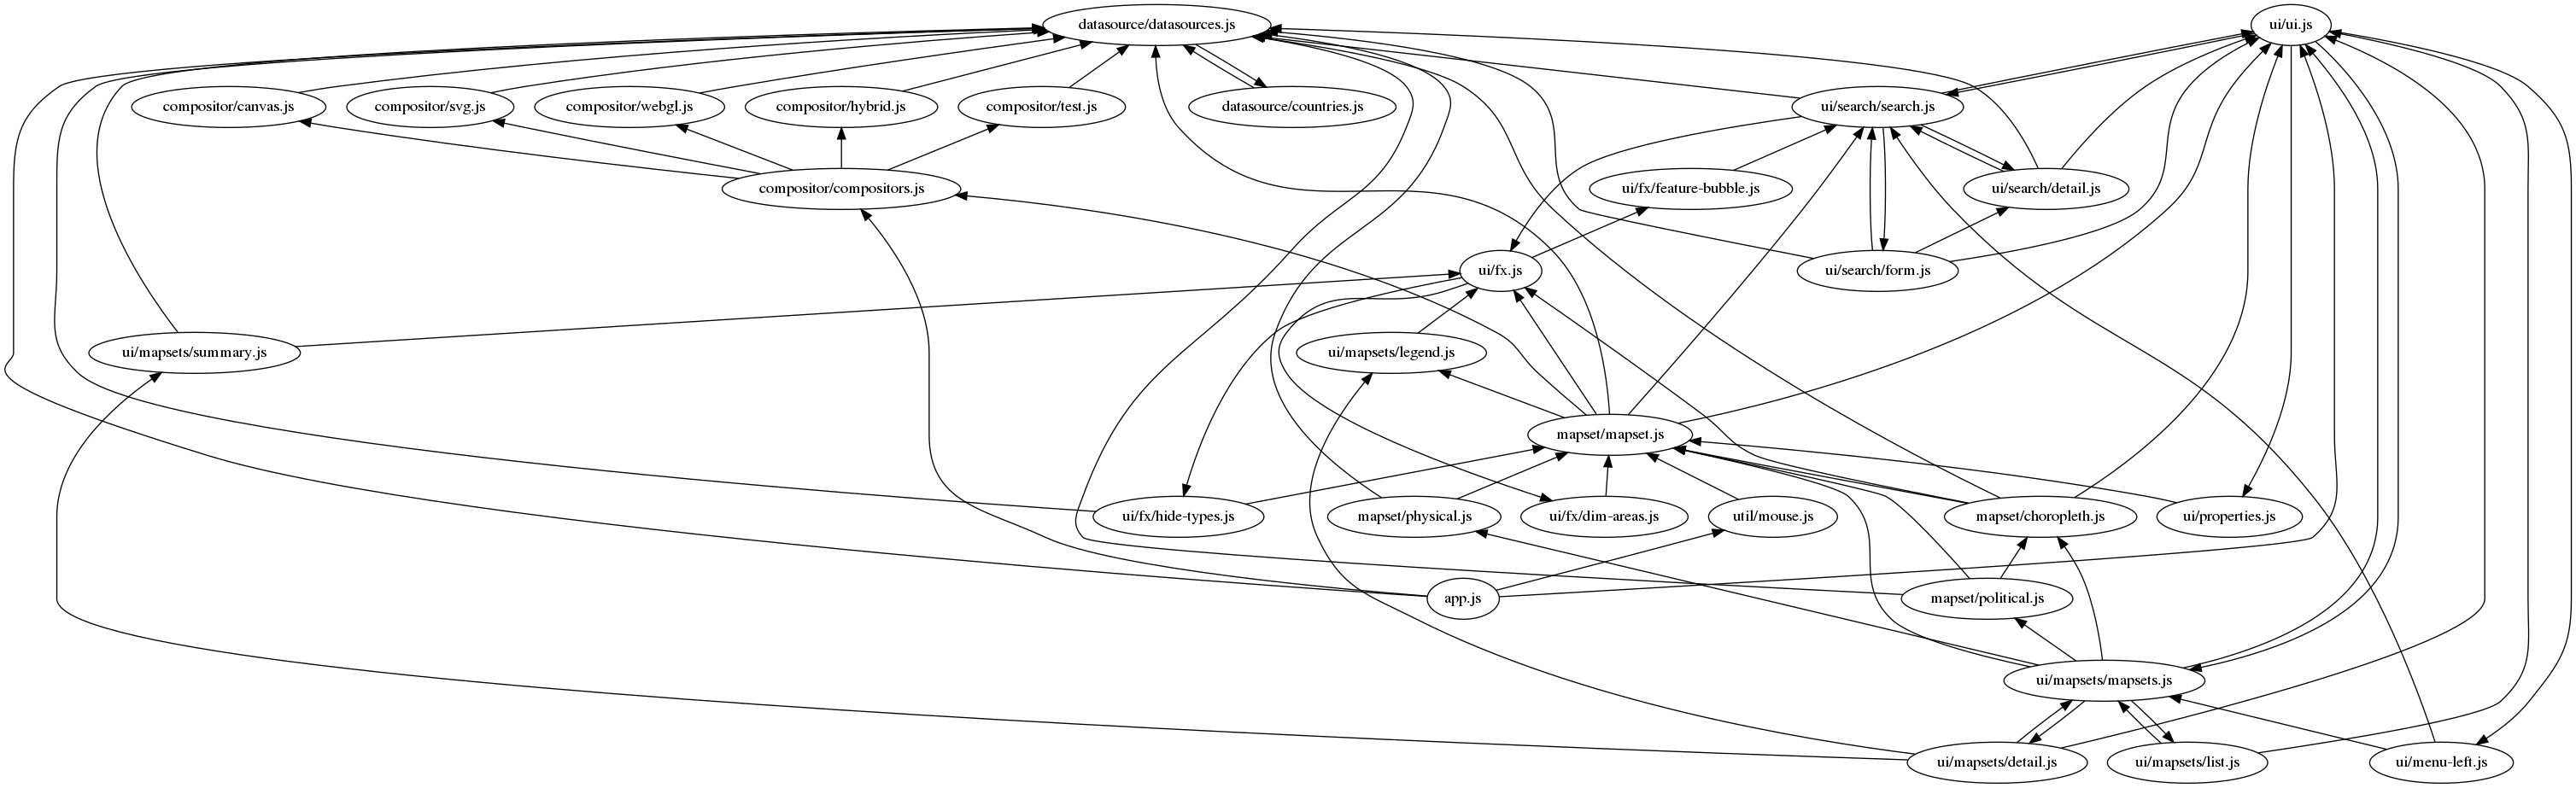
\includegraphics[width=\linewidth]{img/dependency-graph.png}}
	\caption{Visulaisierung eines Dependency-Graphen mit zirkulären Abhängigkeiten. \cite{GraphViz}}
	\label{fig:GraphViz}
\end{figure}
 All diese Elemente dienen als Grundlage zu der Idee, dass zur Risikoeinschätzung der Auswirkungen eines Fehelerfalls innerhalb einer Microsericearchitektur ein ähnlicher Dependency-Graph eine große Hilfe darstellen würde. Baut man den Graphen so auf, wie in obiger Analogie beschrieben, so erhält man einen Graphen, welcher Anzeigt ob und wie weit bestimmte Microservices miteinenander kommunizieren oder sogar voneinander Abhängigkeit sind. Dies beitet die Möglichkeit wertvolle Einblicke in das \textit{makroskopische} Zusammenspiel der einzelnen Komponenten einer Architektur zu erhalten. Ein Softwarearchitekt hat nun die Möglichkeit bei der Entscheidung über die Einführung eines neuen Service Informationen aus ebendiesem Graphen zu nutzen, um festzustellen ob eine zu Starke Abhängikteit zwischen Services vorhanden ist, oder ob es bei der Entwicklung bereits bestehende Abhängigkeiten gibt.
\marginpar{Hier eventeuell bissjen über Kopplung auf Codebassis labern wie das Auswirkungen auf Arhcitektur haben kann} 
Der beschriebene Graph kann also als eine Art Service-Registry angesehen werden, welche Informationen zu der Beziehung zwischen verschiedenen Services beinhaltet. Gleichzeitig wird dadurch vor allem der Bereich der Microservice-Gouvernance betreten, wo eine Service-Registry eine zentrale Komponente darstellt. 

Zusammenfassend lässt sich das Konzept also folgendermaßen beschreiben: \\
Eine Schnittstelle zwischen Microserice-Gouvernance und -Observability wird mithilfe eines Dependency-Graphen gebildet. So spielen Aspekte einer Service-Registry und Elemente des Distributed-Tracing eine große Rolle in diesem Ansatz. 
\chapter{Idee und POC eines Microservice-Dependency Graphen}

Nun, da Grundlegende Begriffe geklärt wurden, werden Kriterien heruasgeabreitet, welche zur spätere Einschätzung und Bewertung eines vorgeschlagenen Ansatzes diesen sollen. Gleichzeitig werden diese Kriterien genutzt, um beretis bestehende Ansätze zu untersuchen und auf ihre Anwendbarkeit zu überprüfen.

Im Rahmen der Observability stehen drei große Säulen im Fokus:
\begin{enumerate}
	\item Logging
	\item Tracing
	\item Metriken
\end{enumerate}

Diese drei Elemente spielen eine wichtige Rolle um eine Lösung im Bereich der Observability liefern zu können. Im Rahmen dieser Arbeit wird vor allem ein Augenmerk auf den Status einer Microserice-Archtitektur gelegt, welche nicht zum Ziel hat, die softwaretechnische Ursache des Problems zu finden, sondern den Service oder den Container zu identifizieren, welcber für den Ausfall veranwtortlich ist. Gleichzeitig gibt es die Anforderung, dass die Abhängigkeiten verschiedener Microservices voneinander dargestellt und in Form von nutzbaren, auswertbaren Daten vorliegen. Hierbei kommt allerdings ein Punkt der Observability zu tragen, da dies, wie später näher erläutert wird auch mithilfe von Tracing erreicht werden kann.\\
Außerdem muss es möglich sein, die gewonnen Daten nutzbar zu machen, um nicht nur feststellen zu können, wecher Service die Ursache des Problems ist, sonder auch, um die Auswirkungen auf andere Services feststellen zu können. Es muss also ein einfacher Weg geschaffen werden, damit die Auswirkungen eines Fehlers schnell festgestellt werden können. 

\chapter{Bewertung und Einschätzung der Arbeit, sowie Ausbilck auf künfitge Arbeiten}
%	Literaturverzeichnis
\clearpage
\ihead{}
\printbibliography[title=Literaturverzeichnis]
\cleardoublepage

% Der Anhang beginnt hier - jedes Kapitel wird alphabetisch aufgezählt. (Anhang A, B usw.)
% \appendix
% \ihead{\appendixname~\thechapter} % Neue Header-Definition

% Ehrenwörtliche Erklärung ewerkl.tex einziehen
% !TEX root =  master.tex

\clearpage
\chapter*{Ehrenwörtliche Erklärung}

% Wird die folgende Zeile auskommentiert, erscheint die ehrenwörtliche
% Erklärung im Inhaltsverzeichnis.

% \addcontentsline{toc}{chapter}{Ehrenwörtliche Erklärung}
Ich versichere hiermit, dass ich die vorliegende Arbeit
 mit dem Thema: \textit{\DerTitelDerArbeit} selbstständig verfasst und keine anderen als die angegebenen Quellen und
Hilfsmittel benutzt habe. Ich versichere zudem,
dass die eingereichte elektronische Fassung mit der gedruckten Fassung übereinstimmt.

\vspace{3cm}
Mannheim, \today \hfill \DerAutorDerArbeit



\end{document}
